\documentclass[10pt,red]{beamer} 
% change the alerted colour to blue
\setbeamercolor{alerted text}{fg=blue}

\usetheme{berlin}
% theme split
\usepackage{beamerthemesplit}

\usepackage{booktabs,array,}
\usepackage{listings}
\usepackage{hyperref}
\usepackage{verbatim,moreverb}
\usepackage{tikz}

\usepackage{color}

\definecolor{dkgreen}{rgb}{0,0.6,0}
\definecolor{gray}{rgb}{0.5,0.5,0.5}
\definecolor{mauve}{rgb}{0.58,0,0.82}

\lstset{frame=tb,
  language = Java,
  aboveskip=3mm,
  belowskip=3mm,
  showstringspaces=true,
  columns=flexible,
  basicstyle={\small\ttfamily},
  numbers=none,
  numberstyle=\tiny\color{gray},
  keywordstyle=\color{blue},
  commentstyle=\color{dkgreen},
  stringstyle=\color{mauve},
  breaklines=true,
  breakatwhitespace=true
  tabsize=4
}
% theme shadow
\usepackage{beamerthemeshadow}

% For including figures
\usepackage{graphicx}

% logo
\logo{
\includegraphics[height=1cm]{iitblogo.pdf}}


% sf family, bold font
\sffamily \bfseries
% Beginning of title page
\title
% content inside [] appears at bottom of all page. content inside {} appears on first page as title. double backslash means line change 
[
	Raspberry Pi Hardware Development	% bottom
	\hspace{0.5cm}
	\insertframenumber/\inserttotalframenumber
]
{
	Interfacing Analog to Digital Converter IC
}

\author
[
	www.e-yantra.org
]
{
	e-Yantra Team \\
  Embedded Real-Time Systems Lab\\
  Indian Institute of Technology-Bombay \\
}
\date
{
IIT Bombay \\ {\today}
}
 
 
\begin{document} 

% Slide-1: Title Page
\begin{frame}
	\titlepage
\end{frame}
\section{ADC converter} 
\begin{frame}
	\frametitle{ADC Converter} \pause
	\begin{enumerate}
		\item<+-|alert@+> An analog-to-digital converter is a device that converts a continuous physical quantity to a digital number.
		\item<+-|alert@+> The Raspberry Pi has no built in analogue inputs.
		\item<+-|alert@+> So, to interface proximity sensors, sharp sensor, temperature sensor.
		\item<+-|alert@+> We need an ADC Converter.
		\item<+-|alert@+> In this tutorial we are using MCP3008 ADC IC.
	\end{enumerate}
\end{frame}
\begin{frame}
	\frametitle{About MCP3008} \pause
	\begin{enumerate}
		\item<+-|alert@+> MCP3008 is a successive approximation 10bit 8-channel Analog to Digital converter (ADC).
		\item<+-|alert@+> It uses the SPI bus protocol which is supported by the RPi header.
	\end{enumerate}
\end{frame}
\begin{frame}
	\frametitle{PINS of MCP3008} \pause
	\centering
	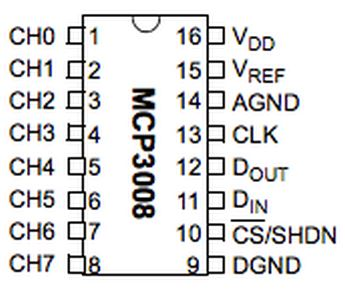
\includegraphics[scale=0.7]{mcp3008}
\end{frame}
\begin{frame} 
	\frametitle{Experiment} \pause
	\textbf{Connect the LM35 temperature sensor to Channel 0 of MCP3008}
\end{frame}
\begin{frame}
	\frametitle{Hardware Required} \pause
		\begin{tabular}{c c c }
				1 & Breadboard &  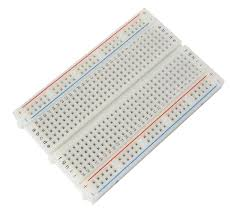
\includegraphics[scale=0.3]{breadboard}
				\vspace{0.3cm}  \\ \pause
				2 & MCP3008 IC. & 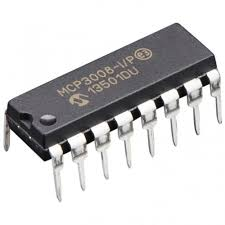
\includegraphics[scale=0.2]{mcp3008_fig}
				\vspace{0.3cm} \\ \pause
			    3 & LM35 Temperature sensor &  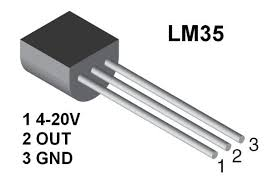
\includegraphics[scale=0.2]{lm35}  
		\end{tabular}
\end{frame}
\subsection{Problem Statement} 
\begin{frame}
	\frametitle{Problem Statement} \pause
	\textbf{ Interfacing an ADC with RPi to read the room temperature using LM35 (Temperature Sensor) connected to one of the channels of IC.}
\end{frame}
\begin{frame}
	\hskip4cm
	\textbf{\LARGE Thank You!} \\[20pt]
	\hskip3cm
	\scriptsize Post your queries on: 
	\hyperref[www.e-yantra.org]{\color{blue} http://qa.e-yantra.org/ \color{black}} 
\end{frame}
\end{document}